%!TEX root = ../../../main.tex
%%---------------------------------------------------------------------------
\section{Vision}
\label{sec:rc_hmi_sec}
%%---------------------------------------------------------------------------
The vision node has the role of detecting LEGO bricks on the conveyor belt using the camera. The detection of brick includes the color, size, position and orientation. This is information that is needed in order to determine whether the brick is needed or not and how to grasp it. 

The vision LEGO detection algorithm is custom made and consists of several elements from the world of vision. Figure \ref{fig:rc_vision_steps_thor} shows the steps performed on an image in order to search for bricks. These steps are described next.\\
	
	\begin{figure}[H]
		\centering
	    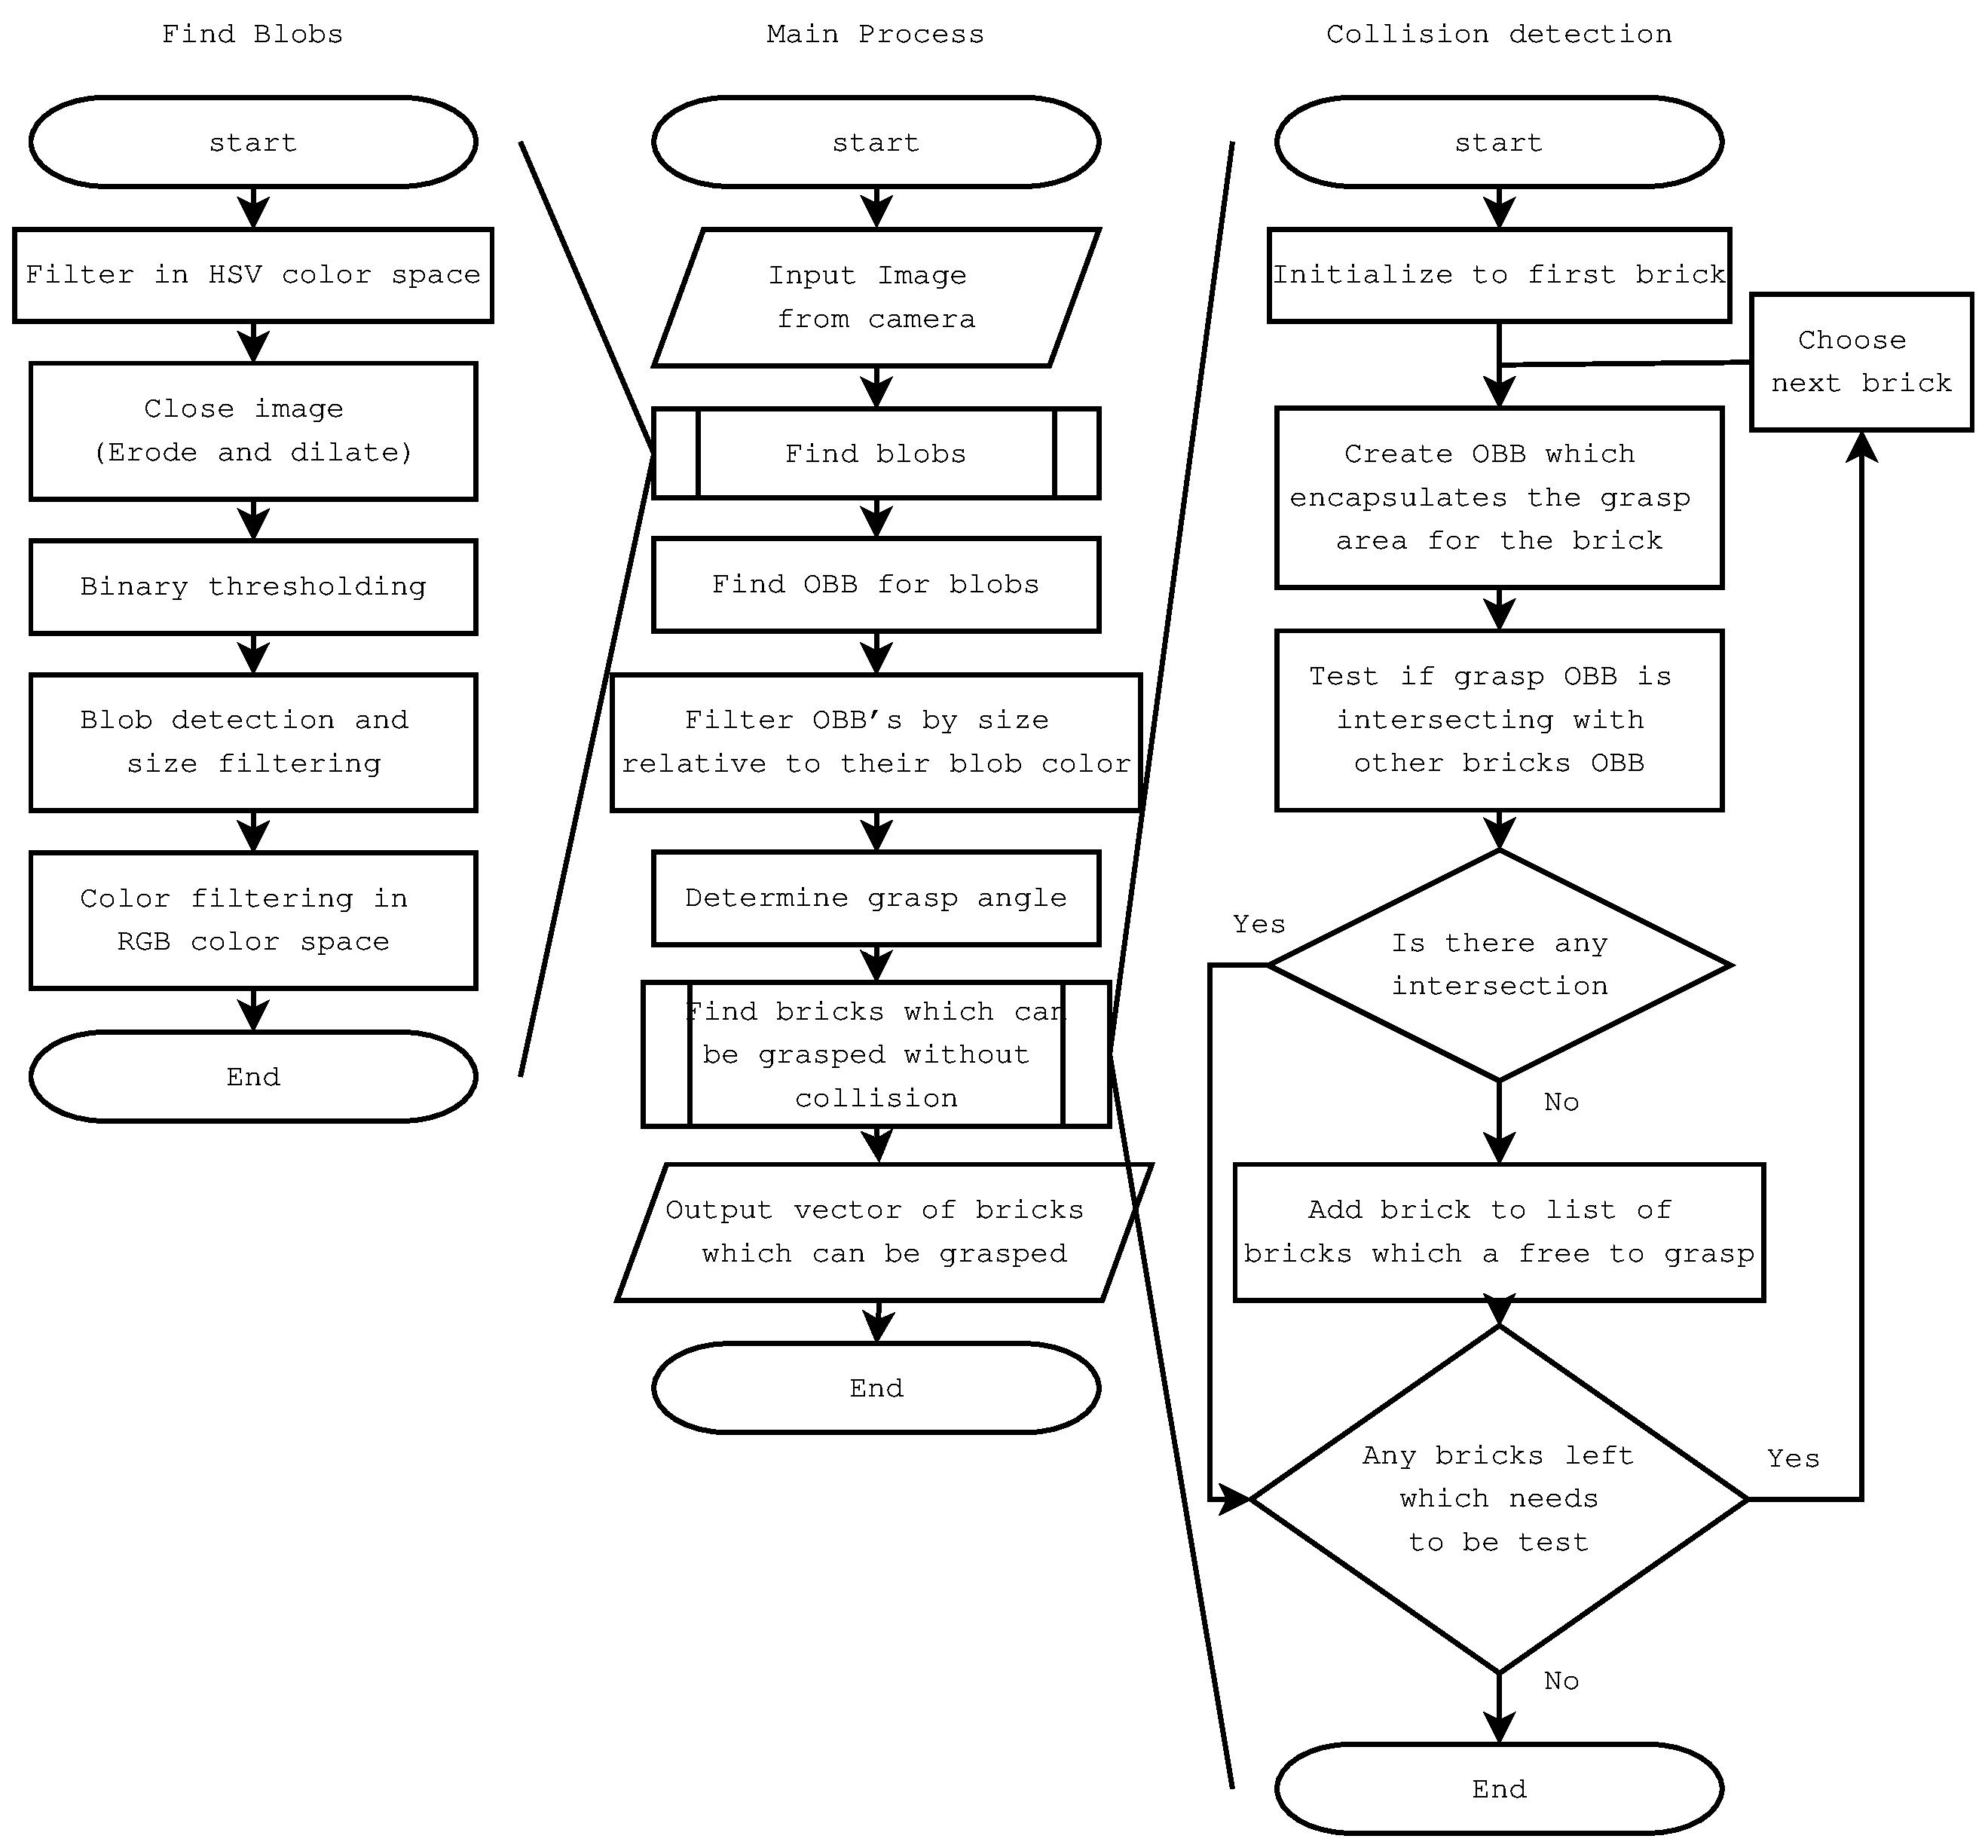
\includegraphics[width=1.0\textwidth]{rc_vision_thor.eps}
	    \caption{Steps to be performed when an image is searched for LEGO bricks}
		\label{fig:rc_vision_steps_thor}
	\end{figure}
	
The vision node is able to deliver two services. One that uses a quick method to tell whether or not any bricks can be seen in the image and one that describes the image in full detail with all relevant brick information. This is used in order to save calculation time since there is no need to request the full vision algorithm if there is no bricks.

The quick method consists of only the left \textit{find blobs} part in figure \ref{fig:rc_vision_steps_thor}. This involves filtering in HSV space in order to separate the background elements from the LEGO bricks. Then the image is \textit{closed} which consists of the erode and dilate process. A binary threshold is applied in order to get a binary representation of the image which is needed in blob detection. The blob detection algorithm detects the connected pixels in the image and separates them as blobs. The blobs are size filtered in order to get rid of small noisy contours. Lastly the color of the blob is determined by a custom color detection algorithm. The average RGB pixel value of all the pixels belonging the blob is calculated and the amount that the respective colors present in percentage with respect to the sum determine the correct color. Looking at the amount that the colors make up, a conclusion of the color can be made. This is robust with respect to changing light conditions and other changes to the colors. 

The next step looks into fitting oriented-bounding-boxes (OBB) to the blobs, using an OpenCV\cite{opencv} implementation. This results in the size, orientation and center position of the detected element. The size and color combination is used for further brick filtering.

The orientation of the bricks is always with respect to the y-axis of the frame and smallest side of the bricks. This makes it easy for grasp calculation and the smallest side is chosen since some LEGO bricks can be too large for grasping on the longest side. 
	
	\begin{figure}[H]
		\centering
	    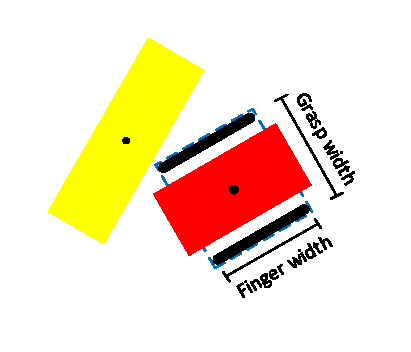
\includegraphics[width=0.5\textwidth]{rc_vision_collision.pdf}
	    \caption{LEGO brick collision detection method}
		\label{fig:rc_vision_collision}
	\end{figure}
	
Finally collision avoidance is done by testing if any obstacles is in the grasp path for a brick. The grasp path for a brick is the area the two fingers of the end effector travels when trying to grasp the brick. Figure \ref{fig:rc_vision_collision} shows a example where the two bold black lines illustrates the end effector fingers. The area encapsulated by the stripped blue lines is the grasp path area for the grasp when trying to grasp the red brick illustrated by a red rectangle. A grasp path area is then tested against all other bricks except the brick to be grasped. Separating axis theorem\cite{Gottschalk:1996:OHS:237170.237244} is used to test if the rectangular grasp area is colliding with the rectangular brick areas defined by OBB's.

Since the positions of the bricks are found in the image and thus in pixels, it needs to be translated to the distance metric that the robot and gripper are using, namely meters. The pixel to meter conversion was archived using a simple method in which four corner points were marked on the conveyor and the distance between these was measured. The same distance was measured on the image in pixels. The different measurements was summed and the average scale found. It was assumed that if the set-up was kept static the scale would be valid for a longer period.

Figure \ref{fig:rc_vision_ex1} and \ref{fig:rc_vision_ex2} shows two results of the vision algorithm. The white box defines the area that a brick can be picked within. The contour of a detected brick is drawn with the color detected. The width of the contour if either thick or thin. Thick illustrates that the brick is pick-able thus not in collision and within the workspace. The green color marks a \textit{monster}, a brick or collection of bricks that is not detected as a valid brick. 

  	\begin{figure}[H]
        \centering
        \begin{subfigure}{0.45\textwidth}
            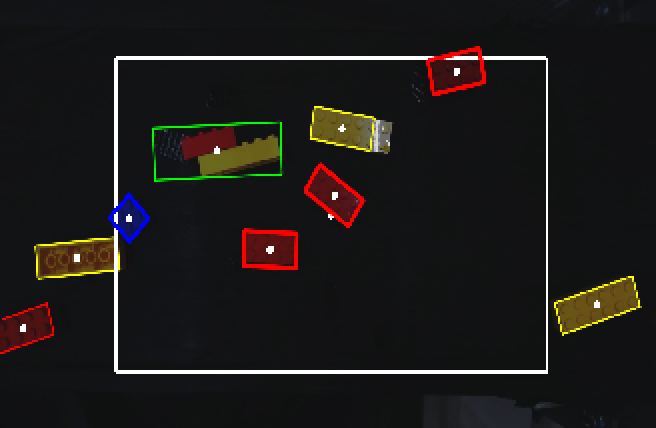
\includegraphics[width=\textwidth]{figs/rc_vision_ex1}
            \caption{}
            \label{fig:rc_vision_ex1}
        \end{subfigure}
        \hspace{10pt}
        \begin{subfigure}{0.45\textwidth}
            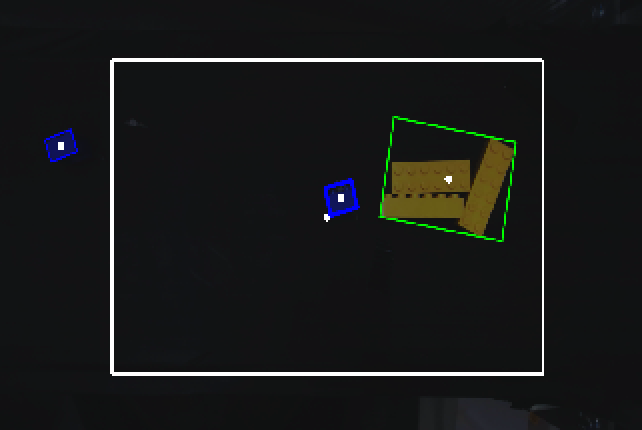
\includegraphics[width=\textwidth]{figs/rc_vision_ex2}
            \caption{Two blue bricks and a \textit{monster}}
            \label{fig:rc_vision_ex2}
    \end{subfigure}
    \caption{Example of vision output}
    \end{figure}